\documentclass[dvipdfmx]{jarticle}

\usepackage[letterpaper,top=2cm,bottom=2cm,left=3cm,right=3cm,marginparwidth=1.75cm]{geometry}
\usepackage{itembkbx}
\usepackage{boites,boites_exemples}
\usepackage{lipsum}
% Useful packages
\usepackage{amsmath}
\usepackage{graphicx}
\usepackage[colorlinks=true, allcolors=blue]{hyperref}
\usepackage{ascmac}
\usepackage[many]{tcolorbox}
\tcbuselibrary{breakable, skins, theorems}
\usepackage{color}
\usepackage{xcolor}
\usepackage{listings}
\lstset{%
  language={Python},
  basicstyle={\small},%
  identifierstyle={\small},%
  commentstyle={\small\itshape\color[rgb]{0,0.5,0}},%
  keywordstyle={\small\bfseries\color[rgb]{0,0,1}},%
  ndkeywordstyle={\small},%
  stringstyle={\small\ttfamily\color[rgb]{1,0,1}},
  frame={tb},
  breaklines=true,
  columns=[l]{fullflexible},%
  numbers=left,%
  xrightmargin=0zw,%
  xleftmargin=3zw,%
  numberstyle={\scriptsize},%
  stepnumber=1,
  numbersep=1zw,%
  lineskip=-0.5ex%
}
\usepackage{tikz}
\usetikzlibrary{shapes.geometric}
\usetikzlibrary {shapes.misc}
\usetikzlibrary{positioning}
\usepackage{algorithmic}
\usepackage{algorithm}
\title{最大公約数の計算}
\author{}
\date{}
\begin{document}
\maketitle
与えられた自然数の集合に対して、共通する約数(公約数)のうちで最大の自然数を最大公約数と呼びます。
ここでは簡単のために二つの自然数$(a,b)$を考えて、その最大公約数${\rm gcd}(a,b)$の計算方法を考えます。
計算のアルゴリズムに入る前に最大公約数の計算例を挙げておきます。
\begin{itemize}
\item 例1\\
	$(52,32)$の最大公約数${\rm gcd}(52,32)$は$52=2^{2}\times 13$と$32=2^5$なので${\rm gcd}(52,13)=4$
\item 例2\\
	$(68,51)$の最大公約数${\rm gcd}(68,51)$は$68=2^{2}\times 17$と$32=3\times 17$なので${\rm gcd}(68,51)=17$
\end{itemize}
最大公約数の計算は以上の例のように小さな数字の組みに対しては比較的簡単にできます。しかし、ある程度数字が大きくなると
機械に頼った計算が必要になってきます。
最大公約数の効率的な計算方法としてユークリッド互除法が古くから知られています。このコードではユークリッド互除法を
使わない愚直な方法とユークリッド互除法を使った方法の二つを実装しています。

\begin{itemize}
\item 愚直な方法\\
最初の方法は、最小公約数は少なくとも与えられた自然数の組み$(a,b)$のうち小さい方の数字$b(<a)$以下である点に注目して、その数字$b$から
初めて$b,b-1,b-2,\cdots$と順番に$a$と$b$が同時に割り切れるかを確認していきます。以下が疑似コードとなります。
\begin{figure}[H]
\begin{algorithm}[H]
	\caption{simple\_gcd}
	\label{alg1}
	\begin{algorithmic}[1]  
	\REQUIRE $a,b$ are positive integer. $(a\geq b)$
    	\STATE $x = b$
    	\IF{$a\%x==0$ and $b\%x==0$}
    	\STATE return $x$
	\ENDIF
    	\STATE $x \leftarrow x-1$
	\STATE goto 2
	\end{algorithmic}
\end{algorithm}
\end{figure}
\item ユークリッド互除法\\
二つ目の方法はユークリッド互除法です。具体的なアルゴリズムの前に以下の点に注目します。
まず与えられた自然数の組み$(a,b)$に対する公約数を$u$とします。するとある自然数$\alpha$と$\beta$を
用いて
\begin{eqnarray}
a&=&\alpha u\\
b&=&\beta u
\end{eqnarray}
と書くことができます。今$a\geq b$としておいて$a$を$b$で割った商をs、余りを$r$とすると
\begin{eqnarray}
r&=&a-bs\\
&=&u(\alpha-\beta s)
\end{eqnarray}
なので$r$も$u$を公約数に持つことがわかります。
また逆に$b$,$r$の公約数を$u'$とするとき
\begin{eqnarray}
b&=&\beta’u’\\
r&=&\gamma'u'
\end{eqnarray}
と書くことができるが
\begin{eqnarray}
a=(\gamma'+\beta' s)u'
\end{eqnarray}
なので$u'$は$a$の公約数でもあります。

この性質を利用して最大公約数を計算するアルゴリズムが以下のユークリッド互除法です。
今、改めて自然の組み$(a,b)$が与えられているとします。$a\geq b$としても一般性は失われません。
$a$を$b$で割った余りを$r_0$とすると$r_0$は$(a,b)$と同じ公約数を持ちかつ$r_0$は$(a,b)$どちらよりも
小さいです。次に$b$を$r_0$で割った余りを$r_1$とします。すると、$r_1$は$b$と$r_0$の公約数と同じ約数を持ち
かつ$r_1$は$b$と$r_0$のどちらよりも小さいです。この作業をくり返いしていくと、以下のような式が得られます。
\begin{eqnarray}
a&=&bq_{0}+r_{1}\\
b&=&r_{1}q_{1}+r_{2}\\
r_1&=&r_{2}q_{2}+r_{3}\\
\cdots\\
r_n&=&r_{n+1}q_{n+1}+r_{n+2}\\
\cdots
\end{eqnarray}
この手続きを繰り返していくことで同じ公約数を持つ数字の列$r_{1}>r_{2}>r_{3}\cdots$が得られ、最終的に
\begin{eqnarray}
r_{m-1}&=&r_{m}q_{m}
\end{eqnarray}
まで行き着きます。この$r_{m}$が求める最大公約数となります。
このユークリッド互除法を疑似コードで書くと以下のようになります。
\begin{figure}[H]
\begin{algorithm}[H]
	\caption{euclidean\_algo}
	\label{alg2}
	\begin{algorithmic}[1]  
	\REQUIRE $a,b$ are positive integer. $(a\geq b)$
    	\STATE $r = a\%b$
    	\IF{$r==0$}
    	\STATE return $b$
	\ENDIF
    	\STATE $a,b = b,r$
	\STATE goto 1
	\end{algorithmic}
\end{algorithm}
\end{figure}
 \end{itemize}
 以上の二つの方法を用いて最大公約数を計算するコードをPythonを用いて実装しました。
 どちらのコードも最大公約数を計算する機能としては同じなのでgcd\_baseという抽象クラスを
 定義してそれを継承するsimple\_gcdとeuclidean\_algoというクラスを作りました。
  \begin{figure}[h]
 \begin{center}
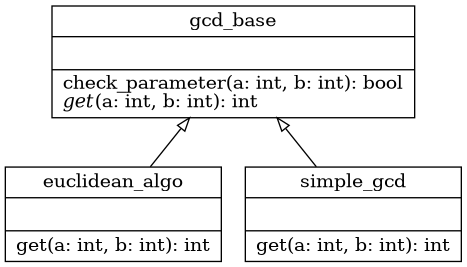
\includegraphics[width=100mm]{classes.png}
\end{center}
\end{figure}
抽象クラスの方では最大公約数を計算する抽象メソッドget(a,b)を宣言しています。
\begin{lstlisting}[caption=gcd\_base,label=base]
class gcd_base(metaclass = ABCMeta):
    def __init__(self)->None:
        pass
    @abstractmethod
    def get(self,a:int,b:int)->int:
        pass

    def check_parameter(self,a:int,b:int)->bool:
        if a<=0 or b<=0:
            print("a and b must be positive!!")
            return False
        return True
 \end{lstlisting}
このgetメソッドは子クラスの方でその実際のアルゴリズムを定義しています。
またcheck\_parameterというメソッドも定義しました。こちらは二つの数字が正の整数かどうか
を判断するメソッドです。このメソッドは子クラスのどのクラスでも共通なので基底クラスの方に
定義しました。

それではこのgcd\_baseクラスを継承したクラスを見ていきます。
\begin{itemize}
\item simple\_gcd
最初のクラスはsimple\_gcdというクラスで実装しました。
\end{itemize}
\begin{lstlisting}[caption=gcd\_simple,label=simple]
class simple_gcd(gcd_base):
    def __init__(self)->None:
        super().__init__()

    def get(self,a:int,b:int)->int:
        if not super().check_parameter(a,b):
            return 0
        if a < b:
            a,b = b,a
        x=b
        while True:
            if a%x == 0 and b%x==0:
                return x
            x-=1
 \end{lstlisting}
 こちらのクラスでは与えられた自然数a,bに対する最大公約数はa,bより小さいことがわかっているので、
 min(a,b)から順番にマイナス1していき最大公約数を計算しています。
 \begin{itemize}
\item gcd\_eucidean
\end{itemize}
二つ目の方法はgcd\_eucideanというクラスで実装しています。
\begin{lstlisting}[caption=gcd\_eucidean,label=euclidean]
 class euclidean_algo(gcd_base):
    def __init__(self)->None:
        super().__init__()

    def get(self,a:int,b:int)->int:
        if not super().check_parameter(a,b):
            return 0
        if a < b:
            a,b = b,a
        while True:
            r = a%b
            if r==0:
                return b
            a,b = b,r
 \end{lstlisting} 
 こちらの方法ではユークリッド互除法を用いて計算しています。
 
 最後にkの二つのアルゴリズムのTATを計測しました。
 \begin{figure}[h]
 \begin{center}
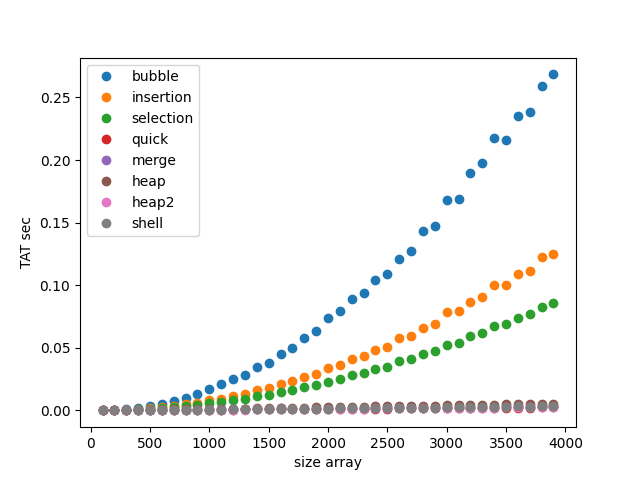
\includegraphics[width=100mm]{time_measure.png}
\end{center}
\end{figure}

\begin{thebibliography}{9}
\item 辻真吾、下平英寿、「Pythonで学ぶアルゴリズムとデータ構造」
\end{thebibliography}

\end{document}
